% 108-09~10(인쇄 108쪽) — 공통 지시문의 두 정규분포곡선 A, B(A 는 왼쪽·낮고 넓게, B 는 오른쪽·높고 좁게 · 대칭축은 점선).
% 스캔 화질이 낮아 TikZ 로 다시 그림. 라벨은 원문에 있는 것만(A, B, x) · 대칭축의 값·대소 관계는 그림에 적지 않는다.
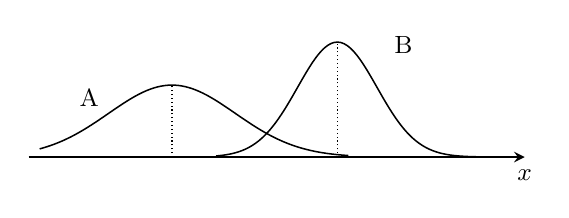
\begin{tikzpicture}[x=0.70cm, y=1.05cm, line width=0.55pt, font=\small]
  \draw[->, >=stealth, line width=0.7pt] (-4.3,0) -- (4.7,0) node[below=1pt] {$x$};
  \draw plot[domain=-4.1:1.5, samples=90, smooth] ({\x},{0.87*exp(-(\x+1.7)*(\x+1.7)/(2*1.15*1.15))});
  \draw plot[domain=-0.9:4.4, samples=90, smooth] ({\x},{1.39*exp(-(\x-1.3)*(\x-1.3)/(2*0.72*0.72))});
  \draw[densely dotted, line width=0.4pt] (-1.7,0) -- (-1.7,0.87);
  \draw[densely dotted, line width=0.4pt] (1.3,0) -- (1.3,1.39);
  \node at (-3.2,0.72) {$\mathrm{A}$};
  \node at (2.5,1.35) {$\mathrm{B}$};
\end{tikzpicture}
